% Poster Figure 3 (Technical Approach, training): three-stage recipe + progressive horizon curriculum.
% Adapted from Fig. training_pipeline and Sec. 3.2.2 in 3_method.tex. Sized for a 10.6in x 6.6in slot.
\documentclass[border=2pt]{standalone}
% Shared style for PRISM figures. Compile with tectonic (XeTeX engine).
\usepackage{lmodern}
\usepackage{amssymb}
\usepackage{fontspec}
\setmainfont{Arial}
\setsansfont{Arial}
\usepackage{amsmath}
\usepackage{booktabs}
\usepackage{colortbl}
\usepackage{xcolor}
\usepackage{tikz}
\usetikzlibrary{arrows.meta,positioning,fit,calc,backgrounds,decorations.pathreplacing}
\usepackage{pgfplots}
\pgfplotsset{compat=1.18}

% PRISM template palette (sampled from the poster template)
\definecolor{prismdark}{HTML}{195A99}
\definecolor{prismmid}{HTML}{1D6FAA}
\definecolor{prismlight}{HTML}{9BB7DC}
\definecolor{prismpale}{HTML}{E8EFF8}
\definecolor{prismaccent}{HTML}{D9822B}
\definecolor{prismgray}{HTML}{6B7280}

\newcommand{\sz}[2]{\fontsize{#1}{#2}\selectfont}
\newcommand{\oursrow}{\rowcolor{prismpale}}
\pgfkeys{/pgf/number format/assume math mode=true}

\begin{document}
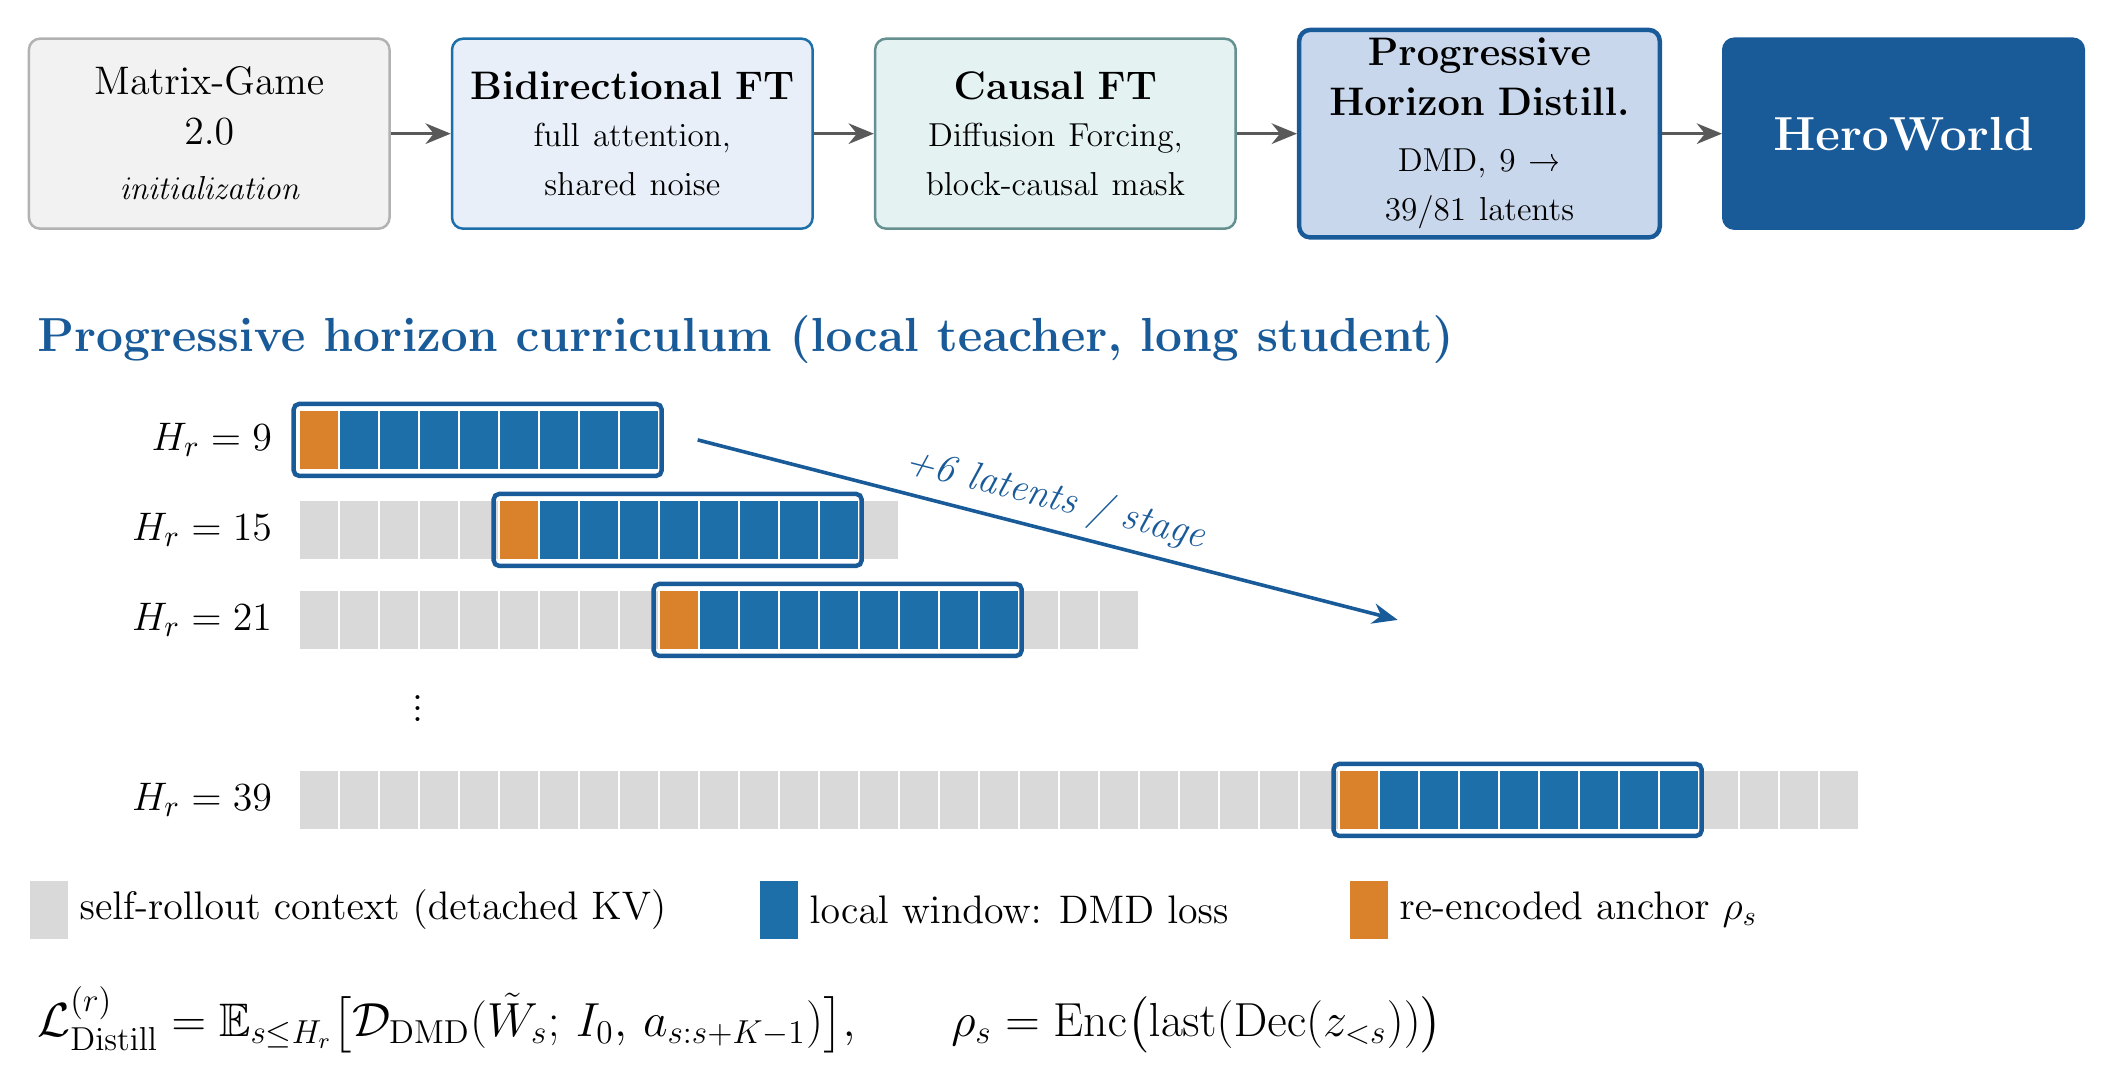
\begin{tikzpicture}[
  font=\sz{15}{18},
  >={Stealth[length=3.2mm,width=2.6mm]},
  stage/.style={rectangle, rounded corners=4pt, line width=0.9pt,
    minimum height=0.95in, text width=1.72in, inner sep=3pt, align=center},
  init/.style={stage, fill=gray!10, draw=gray!60},
  bi/.style={stage, fill=prismpale, draw=prismmid},
  ca/.style={stage, fill=teal!10, draw=teal!55!black!60},
  pr/.style={stage, fill=prismlight!55, draw=prismdark, line width=1.6pt},
  fin/.style={stage, fill=prismdark, draw=prismdark, text=white, font=\sz{18}{21}\bfseries},
  arr/.style={->, line width=1.3pt, draw=black!65},
  cell/.style={rectangle, draw=white, line width=0.8pt, minimum width=0.2in, minimum height=0.3in, inner sep=0pt, anchor=west},
]
% ---- (a) three-stage pipeline ----
\node[init] (s0) at (0,0) {Matrix-Game\\2.0\\[2pt]{\sz{13}{15}\itshape initialization}};
\node[bi, right=0.3in of s0] (s1) {\textbf{Bidirectional FT}\\[2pt]{\sz{13}{15} full attention,\\shared noise}};
\node[ca, right=0.3in of s1] (s2) {\textbf{Causal FT}\\[2pt]{\sz{13}{15} Diffusion Forcing,\\block-causal mask}};
\node[pr, right=0.3in of s2] (s3) {\textbf{Progressive}\\\textbf{Horizon Distill.}\\[2pt]{\sz{13}{15} DMD, 9 → 39/81 latents}};
\node[fin, right=0.3in of s3] (s4) {HeroWorld};
\foreach \a/\b in {s0/s1,s1/s2,s2/s3,s3/s4} \draw[arr] (\a) -- (\b);

% ---- (b) progressive horizon curriculum ----
\coordinate (origin) at ([yshift=-0.55in]s0.south west);
\node[anchor=west, font=\sz{17}{20}\bfseries, text=prismdark] at (origin) {Progressive horizon curriculum (local teacher, long student)};
\def\cw{0.2in}
\def\x0{1.35in}
% rows: horizon H, window start s (0-indexed), row index
\foreach \H/\s/\r in {9/0/0, 15/5/1, 21/9/2, 39/26/4}{
  \pgfmathsetmacro{\y}{-0.5-0.45*\r}
  \node[anchor=east, font=\sz{15}{18}] at ($(origin)+(\x0-0.08in,\y in)$) {$H_r = \H$};
  \foreach \k in {1,...,\H}{
    \pgfmathtruncatemacro{\idx}{\k-1}
    \pgfmathtruncatemacro{\inwin}{(\idx>=\s) && (\idx<\s+9)}
    \pgfmathtruncatemacro{\anchor}{\idx==\s}
    \ifnum\anchor=1 \def\fc{prismaccent}\else\ifnum\inwin=1 \def\fc{prismmid}\else\def\fc{gray!30}\fi\fi
    \node[cell, fill=\fc] at ($(origin)+(\x0+\idx*\cw,\y in)$) {};
  }
  \draw[prismdark, line width=1.6pt, rounded corners=2pt]
    ($(origin)+(\x0+\s*\cw-0.02in,\y in+0.18in)$) rectangle ($(origin)+(\x0+\s*\cw+9*\cw+0.02in,\y in-0.18in)$);
}
\node[font=\sz{18}{18}] at ($(origin)+(\x0+0.6in,-0.5in-0.45*3 in+0.05in)$) {$\vdots$};
% growth arrow
\draw[->, line width=1.3pt, prismdark] ($(origin)+(\x0+2.0in,-0.5in)$) -- node[above, sloped, font=\sz{14}{16}\itshape, text=prismdark] {+6 latents / stage} ($(origin)+(\x0+5.5in,-0.5in-0.45*2in)$);
% legend
\def\ly{-2.85}
\node[cell, fill=gray!30] (l1) at ($(origin)+(0in,\ly in)$) {};
\node[anchor=west, font=\sz{14}{17}] at (l1.east) {self-rollout context (detached KV)};
\node[cell, fill=prismmid] (l2) at ($(origin)+(3.65in,\ly in)$) {};
\node[anchor=west, font=\sz{14}{17}] at (l2.east) {local window: DMD loss};
\node[cell, fill=prismaccent] (l3) at ($(origin)+(6.6in,\ly in)$) {};
\node[anchor=west, font=\sz{14}{17}] at (l3.east) {re-encoded anchor $\rho_s$};
% equations
\node[anchor=west, font=\sz{17}{20}] at ($(origin)+(0in,-3.4in)$)
  {$\mathcal{L}^{(r)}_{\mathrm{Distill}} = \mathbb{E}_{s \le H_r}\big[\mathcal{D}_{\mathrm{DMD}}(\tilde{W}_s;\, I_0,\, a_{s:s+K-1})\big],\qquad
    \rho_s = \mathrm{Enc}\big(\mathrm{last}(\mathrm{Dec}(z_{<s}))\big)$};
\end{tikzpicture}
\end{document}
